\documentclass[11pt,fleqn]{article}
%\usepackage{CJK}
\usepackage{latexsym}
\usepackage{color}
\usepackage{graphicx, float}\usepackage{graphicx}
\usepackage{algorithmic}
\usepackage{algorithm}
%\usepackage{algpseudocode}
%\usepackage[colorlinks]{hyperref}
\usepackage[toc,page]{appendix}
\usepackage{bm}
\setlength{\oddsidemargin}{-0.0in}
\setlength{\evensidemargin}{-0.0in} \setlength{\textwidth}{6.0in}
\setlength{\textheight}{9.0in} \setlength{\topmargin}{-0.2in}
%\usepackage[boxruled]{algorithm2e}

%\setlength{\leftmargin}{0.7in}
\usepackage{amssymb, graphicx, amsmath}  %  fancyheadings,
\usepackage{setspace}
\newcommand\qed{\qquad $\square$}
\newcommand{\nn}{\nonumber}

\usepackage{lipsum}

\def \[{\begin{equation}}
\def \]{\end{equation}}
\def\proof{{\bf Proof:\quad}}
\def \endzm {\quad $\Box$}
\def\dist{\hbox{dist}}

\usepackage{tabularx,booktabs}
\newcolumntype{C}{>{\centering\arraybackslash\hsize=.5\hsize}X} % centered version of "X" type
\setlength{\extrarowheight}{1pt}
\usepackage{caption}% <-- added


\newcommand{\R}{\mathbb{R}}
%\newtheorem{yinli}{����}[section]
\newcommand{\D}{\displaystyle}
\newcommand{\T}{\textstyle}
\newcommand{\SC}{\scriptstyle}
\newcommand{\FT}{\footnotesize}

\usepackage{hyperref}
\newcommand\fnurl[2]{%
  \href{#2}{#1}\footnote{\url{#2}}%
}


%\newtheorem{theorem}{Theorem}[section]
%\renewcommand{\thetheorem}{\arabic{section}.\arabic{theorem}}
\newtheorem{definition}{Definition}
\renewcommand{\thedefinition}{\arabic{section}.\arabic{definition}}
\newtheorem{lemma}{Lemma}[section]
\renewcommand{\thelemma}{\arabic{section}.\arabic{lemma}}
\newtheorem{remark}{Remark}
\renewcommand{\theremark}{\arabic{section}.\arabic{remark}}
\newtheorem{proposition}{Proposition}[section]
\renewcommand{\theproposition}{\arabic{section}.\arabic{proposition}}
\newtheorem{corollary}{Corollary }[section]
\renewcommand{\thecorollary}{\arabic{section}.\arabic{corollary}}
\renewcommand{\theequation}{\arabic{section}.\arabic{equation}}
\renewcommand{\baselinestretch}{1.35}
\newtheorem{exam}{Example}[section]
\renewcommand{\theexam}{\arabic{section}.\arabic{exam}}
\newtheorem{theo}{Theorem}[section]
\renewcommand{\thetheo}{\arabic{section}.\arabic{theo}}

% Define a \HEADER{Title} ... \ENDHEADER block
\makeatletter
\newcommand{\HEADER}[1]{\ALC@it\underline{\textsc{#1}}\begin{ALC@g}}
\newcommand{\ENDHEADER}{\end{ALC@g}}
\makeatother

\newcommand{\argmin}{\operatornamewithlimits{argmin}}
\newcommand{\argmax}{\operatornamewithlimits{argmax}}

\begin{document}
%\begin{CJK*}{GBK}{song}

\begin{center}

{\LARGE \bf CS391L Machine Learning HW6: Deep Learning}\\

\vskip 25pt
 {Zeyuan Hu, iamzeyuanhu@utexas.edu }\\
\vskip 5pt
{\small EID:zh4378 Fall 2017 }

\end{center}

\begin{spacing}{1.5}
\section{Introduction}

\paragraph{}In this task, we are asked to apply the neural networks to \fnurl{handwritten image data}{http://yann.lecun.com/exdb/mnist/} 
to recognize the image identity. The handwritten digit image is described by an $28\times28$ array of brightness values. 
We are given $60000$ exemplars of images with known labels of the digits. Our objective is to 
take a new image and identify the digit in the image. We choose track II and implement a Feedforward 
Neural Network (FFNN) and a Convolutional Neural Network (CNN). We choose these two neural network architectures
because they are known to be effective to the image classification task.

\section{Method}

Both FFNN and CNN are implemented using \fnurl{Keras}{https://keras.io/} framework. The network architectures and hyperparameters are
detailed below.

\subsection{FeedForward Neural Network} 

The architecture of FFNN is shown in Figure \ref{FFNN-Arch}. We implement a network with two hidden layers and the hyperparameters
are shown in Table \ref{FFNN-Config}. We use raw pixel values as input to the network. The images are matrices of size $28\times28$.
Thus, we rehape the image matrix to an array of size 784 (i.e., $28\times28 = 784$) and feed this array to the network. The output
layer will have 10 neurons for the 10 digits. The implementation is rather straightforward. We convert each image matrix to an array
and then we convert the data to float and scale the values between 0 and 1. We then convert the labels from integer to categorical
(i.e., one-hot) vectors. Then, we build the model. Note that we need to prevent the overfitting, which is done by adding dropout for each
layer. Dropout means a fraction of neurons we randomly turn off during the training process.

\begin{figure}
\centering
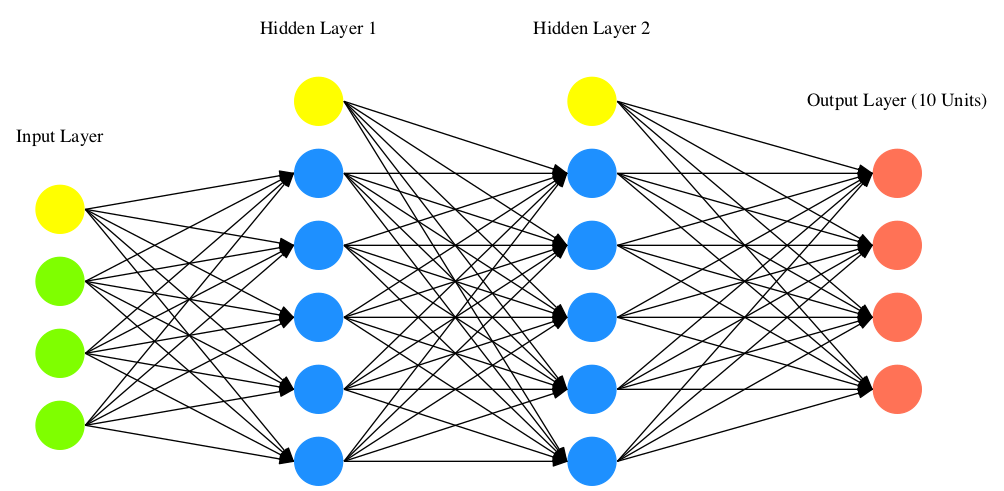
\includegraphics[scale=0.5]{ffnn.png} 
\caption{FeedForward Neural Network Architecture}
\label{FFNN-Arch}
\end{figure}

\begin{table}
\captionsetup{size=footnotesize}
\caption{FFNN Configuration} 
\label{FFNN-Config}
%\setlength\tabcolsep{0pt} % let LaTeX compute intercolumn whitespace
\footnotesize\centering
%This table provides the frequencies.

\smallskip 
\begin{tabular*}{\columnwidth}{@{\extracolsep{\fill}}lc}
\toprule
  Description  & Values  \\
\midrule
 batch size & 256      \\
 number of hidden layer & 2 \\
 number of hidden units for Hidden Layer 1 & 512        \\
 number of hidden units for Hidden Layer 2 & 512  \\
 dropout rate & 0.5 \\
 number of epochs & 20        \\
 learning rate & 0.001        \\
 optimizer & RMSprop \\
\bottomrule
\end{tabular*}
\end{table}

\subsection{Convolutional Neural Network}

The architecture of CNN is shown in Figure \ref{CNN-Arch}. We implement a network with two convolution layers
and one max pooling layer. Then we include dropout to avoid overfitting and we add a dense layer followed by
a softmax layer to get our final classification result. The hyperparameters are shown in Table \ref{CNN-Config}.
The implementation is similar to the FFNN one. The only difference is that we now use CNN instead of FFNN.

\begin{figure}
\centering
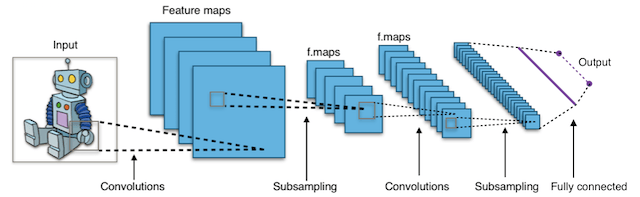
\includegraphics[scale=0.5]{typical_cnn_architecture.png} 
\caption{Convolutional Neural Network Architecture}
\label{CNN-Arch}
\end{figure}

\begin{table}
\captionsetup{size=footnotesize}
\caption{CNN Configuration} 
\label{CNN-Config}
%\setlength\tabcolsep{0pt} % let LaTeX compute intercolumn whitespace
\footnotesize\centering
%This table provides the frequencies.

\smallskip 
\begin{tabular*}{\columnwidth}{@{\extracolsep{\fill}}lc}
\toprule
  Description  & Values  \\
\midrule
 batch size & 128      \\
 number of convolution layer & 2 \\
 number of max pooling layer & 1 \\
 feature maps for convolution layer 1 & 32 \\
 feature maps for convolution layer 2 & 64 \\
 filter region size & (3,3) \\
 pooling region size & (2,2) \\
 dropout rate & 0.5 \\
 number of epochs & 12        \\
 learning rate & 1.0        \\
 optimizer & Adadelta \\
\bottomrule
\end{tabular*}
\end{table}


\section{Results}

The performance of FFNN is shown in Figure \ref{FFNN-loss} and \ref{FFNN-acc}. The accuracy for the test set is 98.36\% and
the loss is 0.079. The accuracy for the test set is 98.98\% and the loss is 0.031.

\begin{figure}
\centering
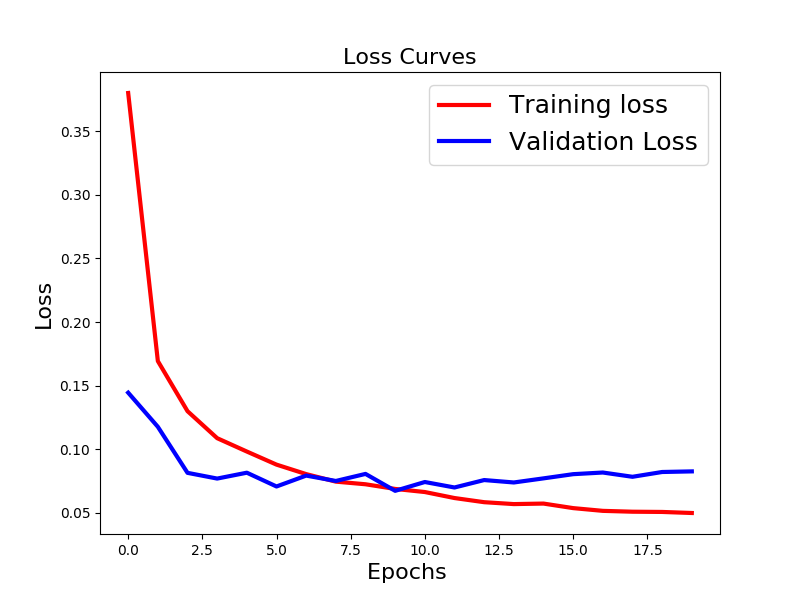
\includegraphics[scale=0.5]{loss-ffnn.png} 
\caption{Loss for Feedfoward Neural Network}
\label{FFNN-loss}
\end{figure}

\begin{figure}
\centering
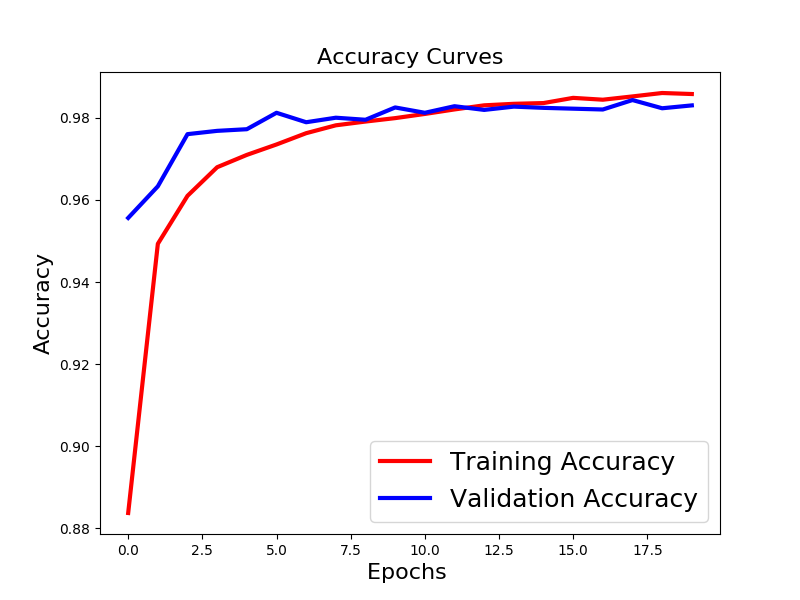
\includegraphics[scale=0.5]{acc-ffnn.png} 
\caption{Accuracy for Feedforward Neural Network}
\label{FFNN-acc}
\end{figure}

\begin{figure}
\centering
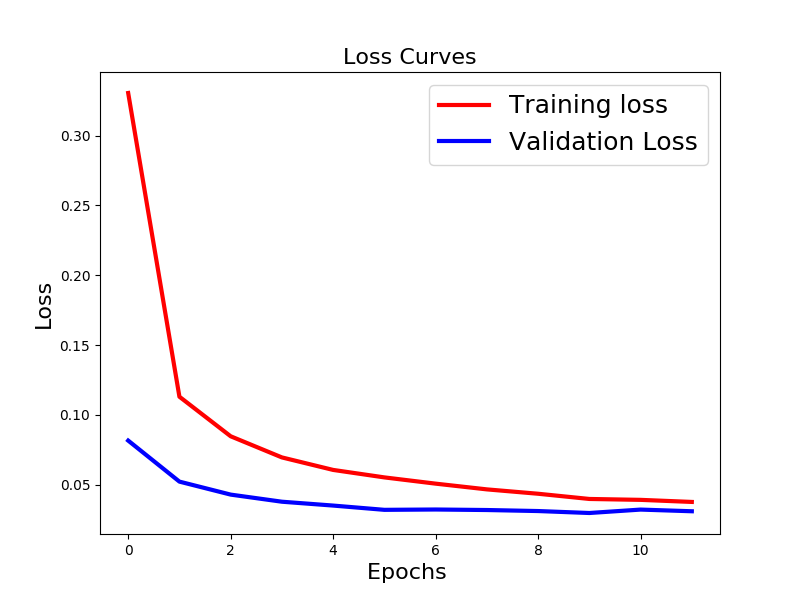
\includegraphics[scale=0.5]{loss-cnn.png} 
\caption{Loss for Convolutional Neural Network}
\label{CNN-loss}
\end{figure}

\begin{figure}
\centering
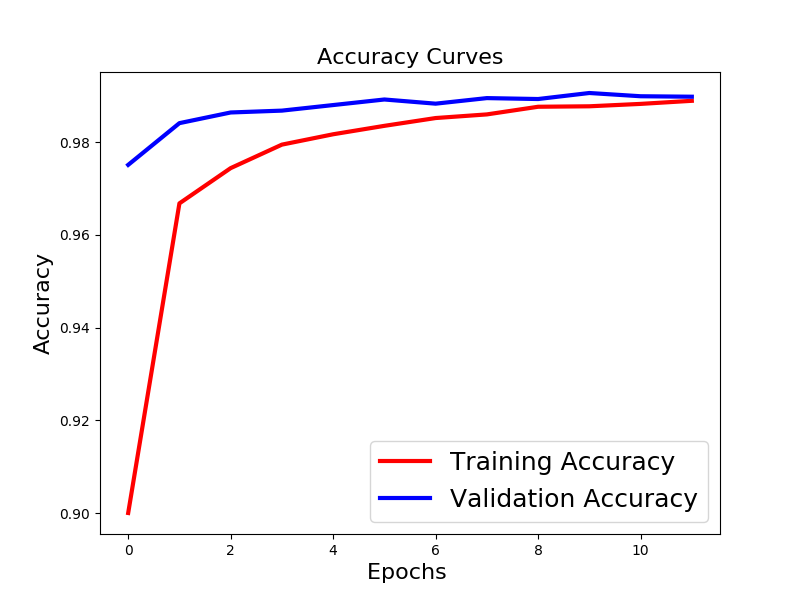
\includegraphics[scale=0.5]{acc-cnn.png} 
\caption{Accuracy for Convolutional Neural Network}
\label{CNN-acc}
\end{figure}

\section{Discussion and Conclusion}

In this task, I implement a FFNN and a CNN for handwritten digit image classification task. As shown by the result, 
the classification accuracy is very high for both the FFNN and CNN. The main reason for neural networks that can have
a good result on this task is that the neural networks are really good at nonlinear classification. In addition, the 
use of dropout prevents us from overfitting, which helps us to achieve a good accuracy on the test set as well.

\end{spacing}

%\bibliographystyle{ieeetr}
%\bibliography{report}

\begin{appendices}

\section{How to run the code}

\paragraph{}To run my code, unzip the \verb|hw6.zip| and get \verb|ffnn.py| and \verb|cnn.py|. Then, you
can run the code with the following commands:

\begin{itemize}
\item \verb|Python ffnn.py|
\item \verb|Python cnn.py|
\end{itemize}

My code is heavily commented and please take a look if there are any type of questions.

\end{appendices}


\end{document}
